\begin{appendix} 
	
\section{Bildschirmfotos}

\hspace{\textwidth}

\begin{figure}[H]
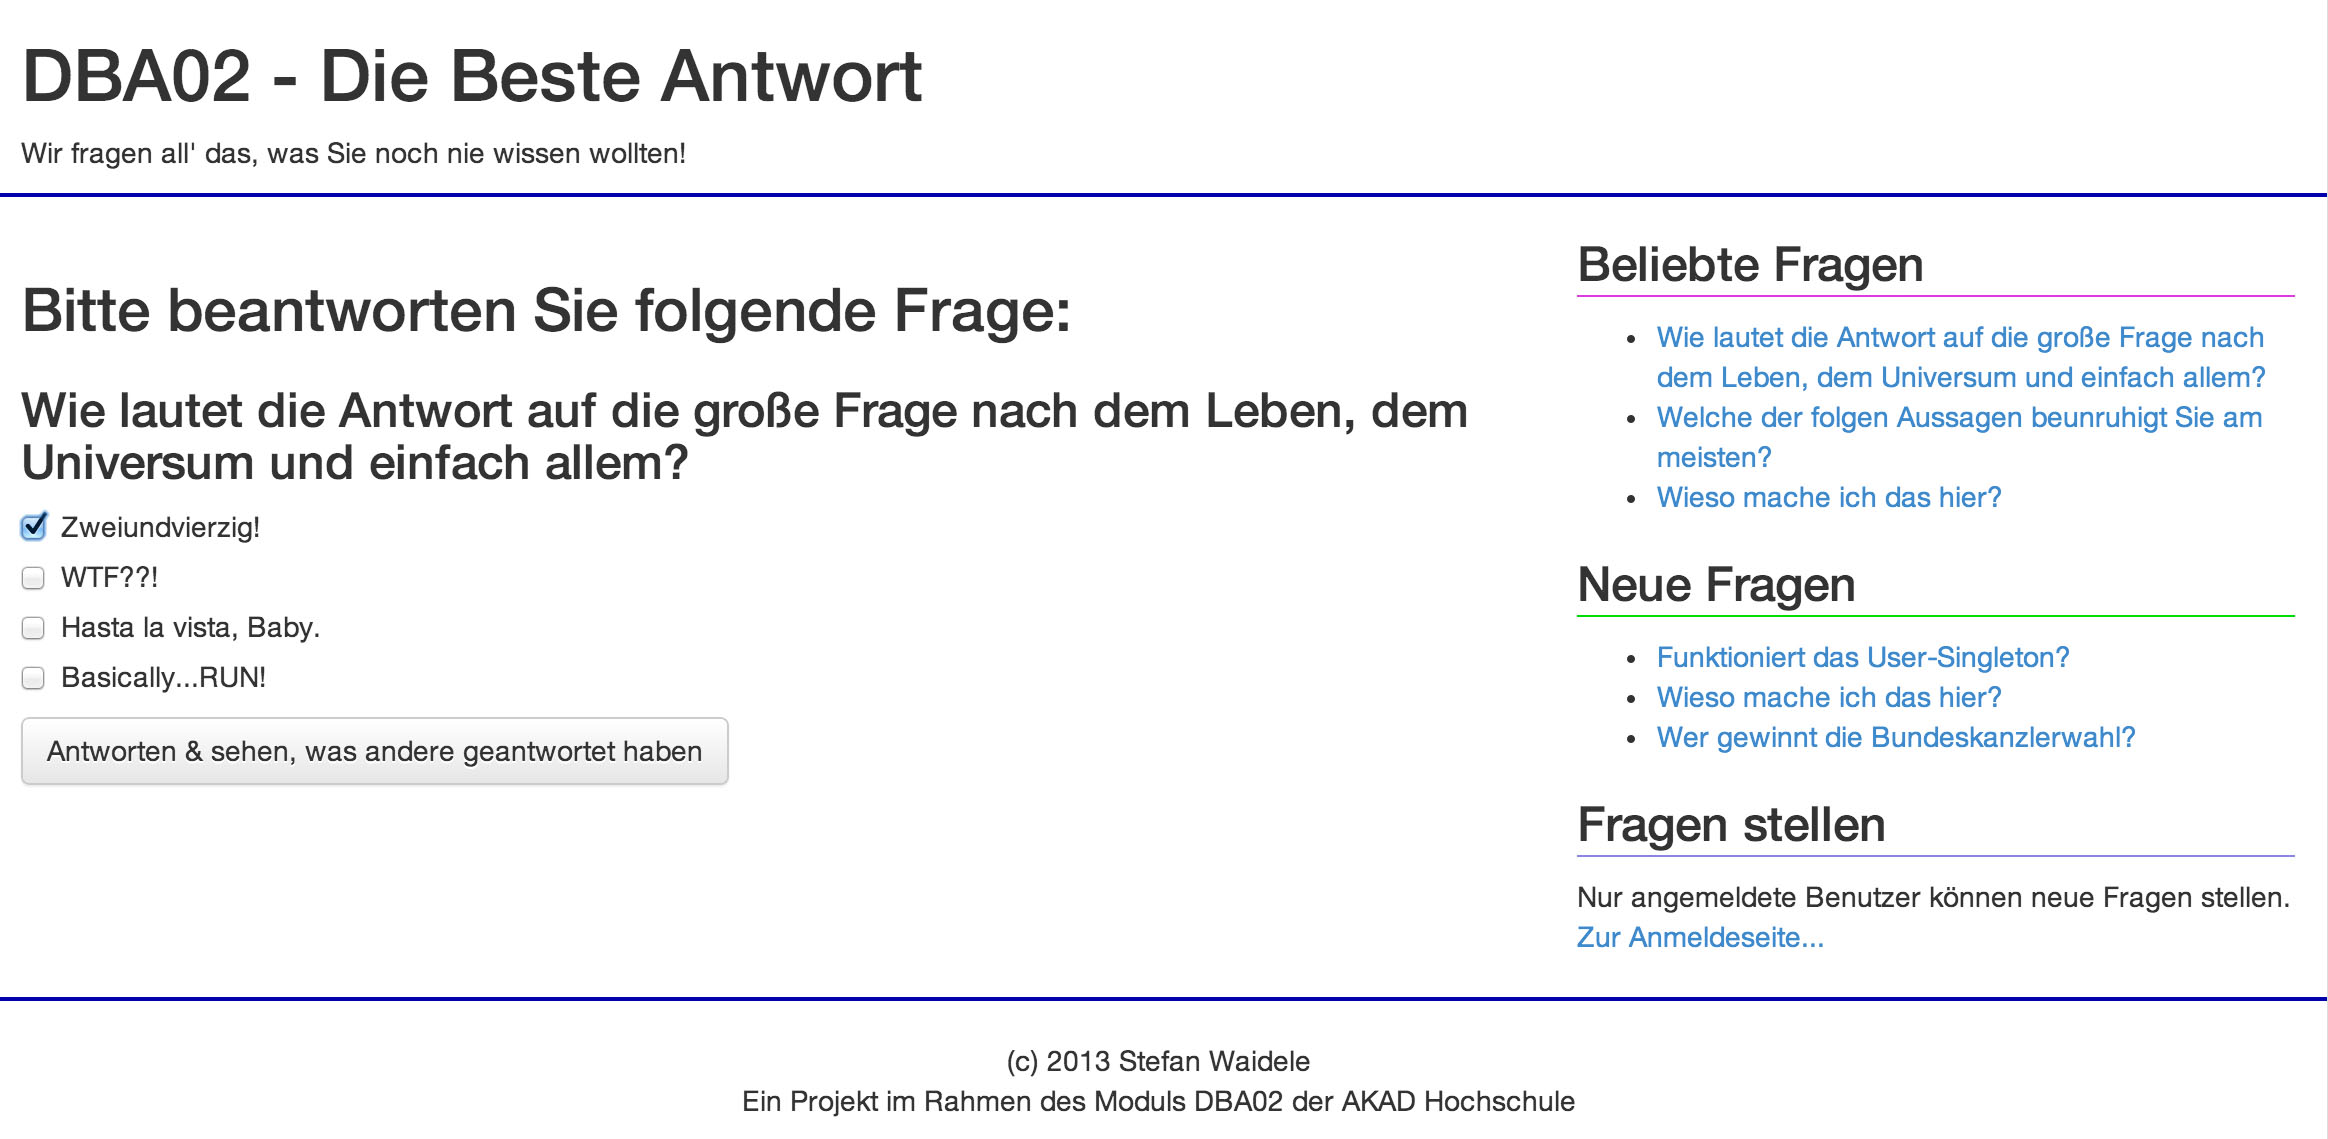
\includegraphics[width=\textwidth]{scr-frage.jpg}
\caption{Screenshot: Frage}
\label{scr:frage}
\end{figure}

\begin{figure}[H]
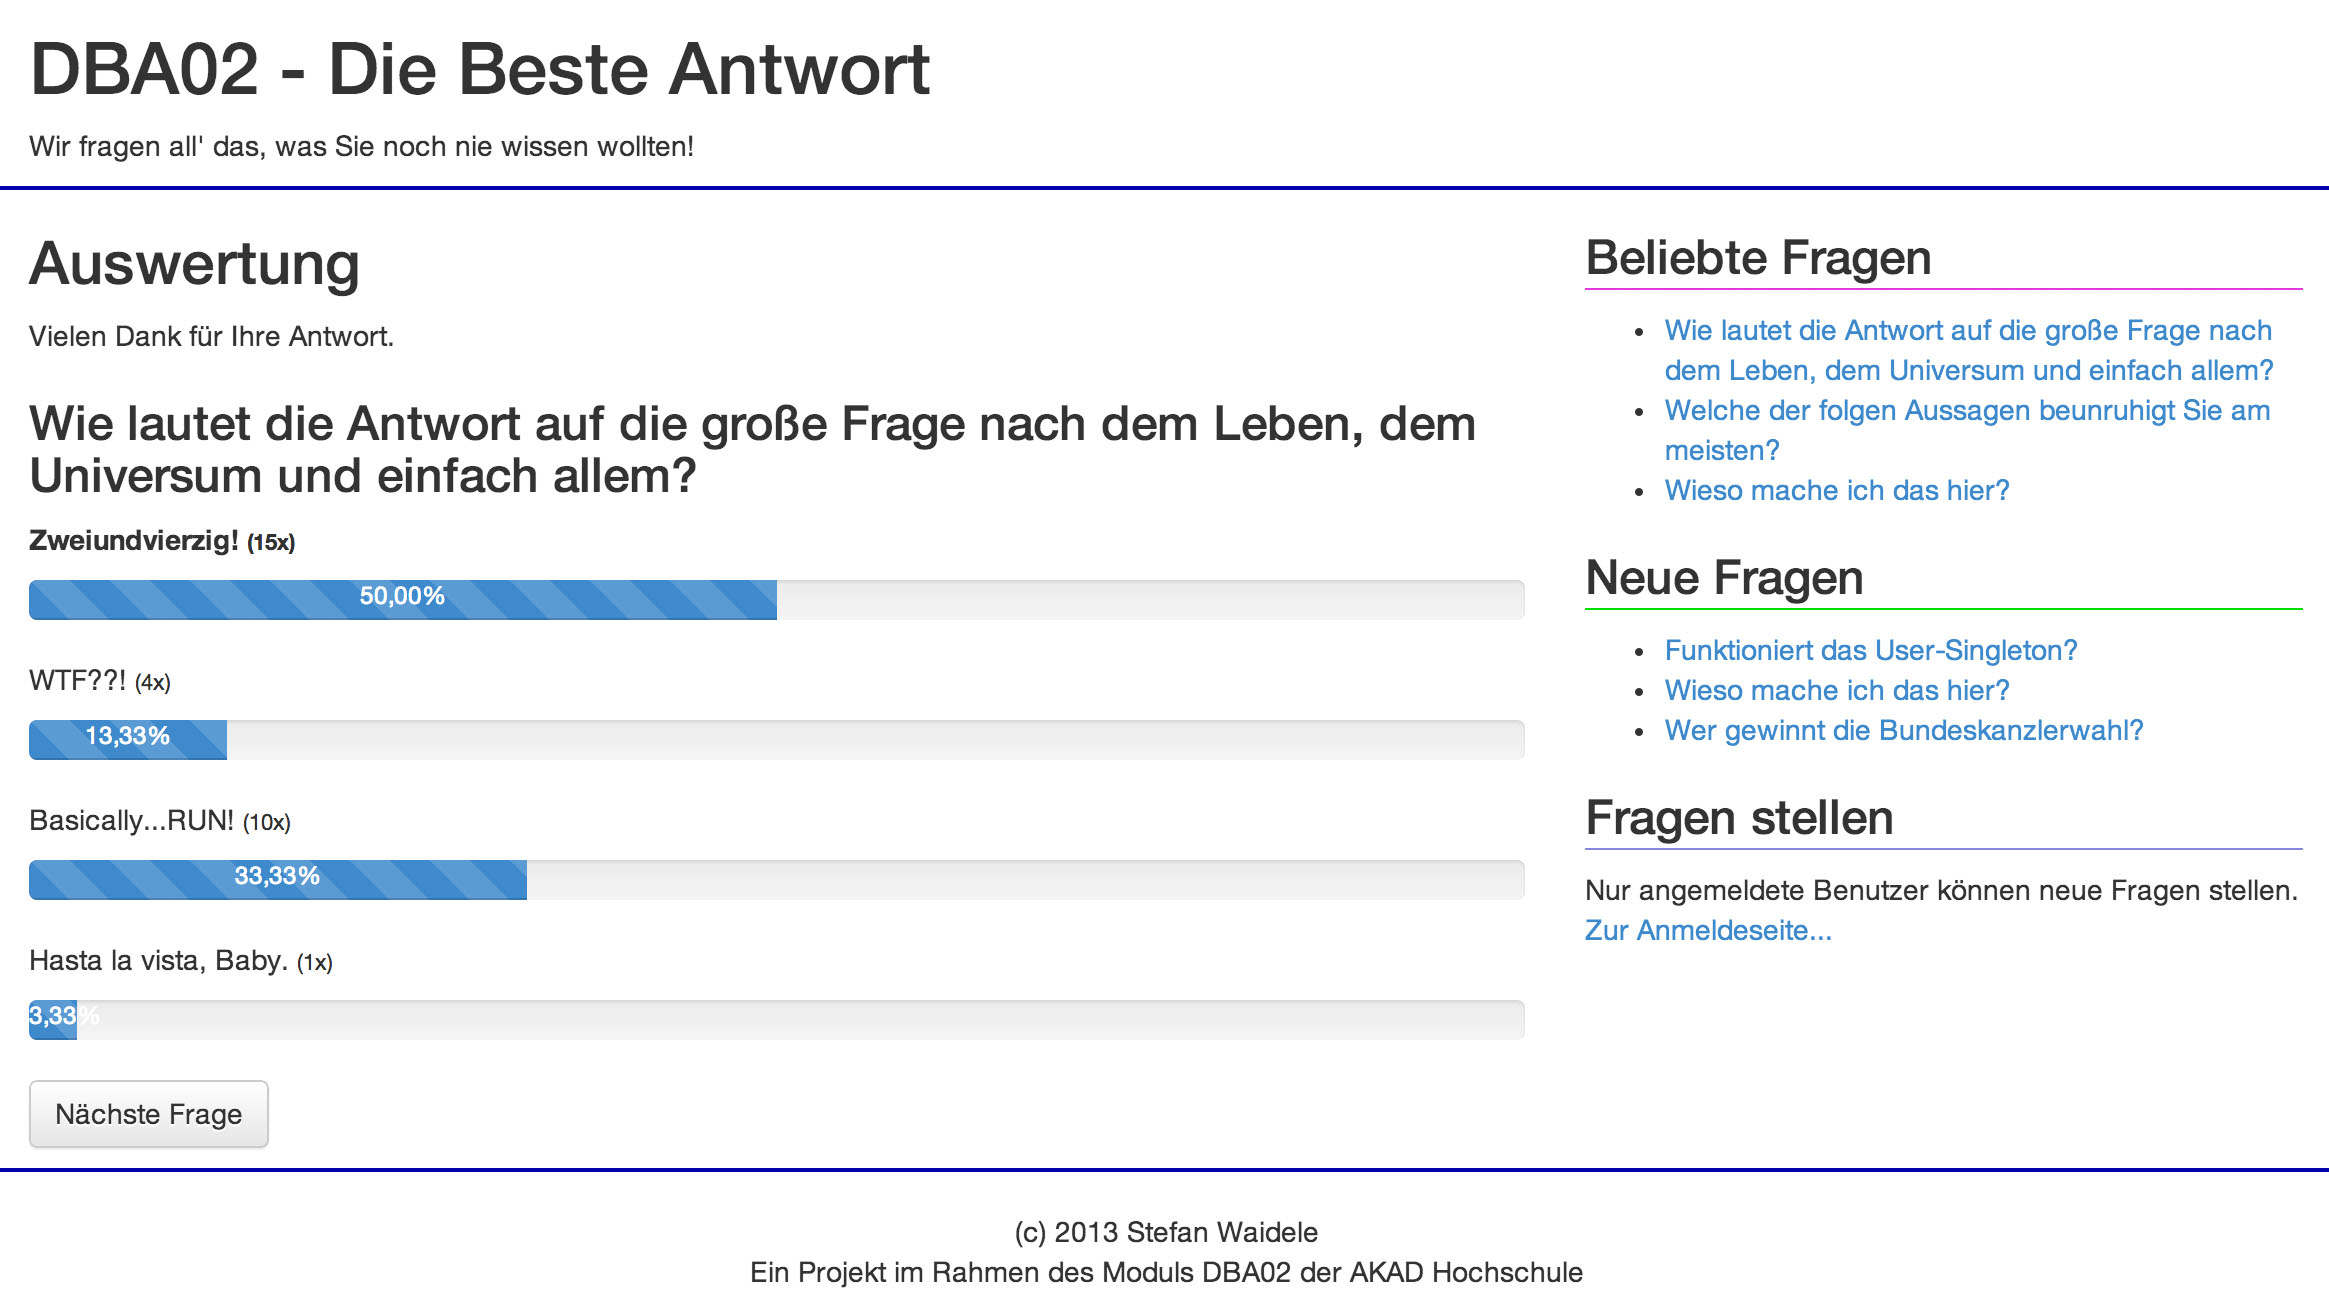
\includegraphics[width=\textwidth]{scr-auswertung.jpg}
\caption{Screenshot: Auswertung}
\label{scr:auswertung}
\end{figure}

\begin{figure}[H]
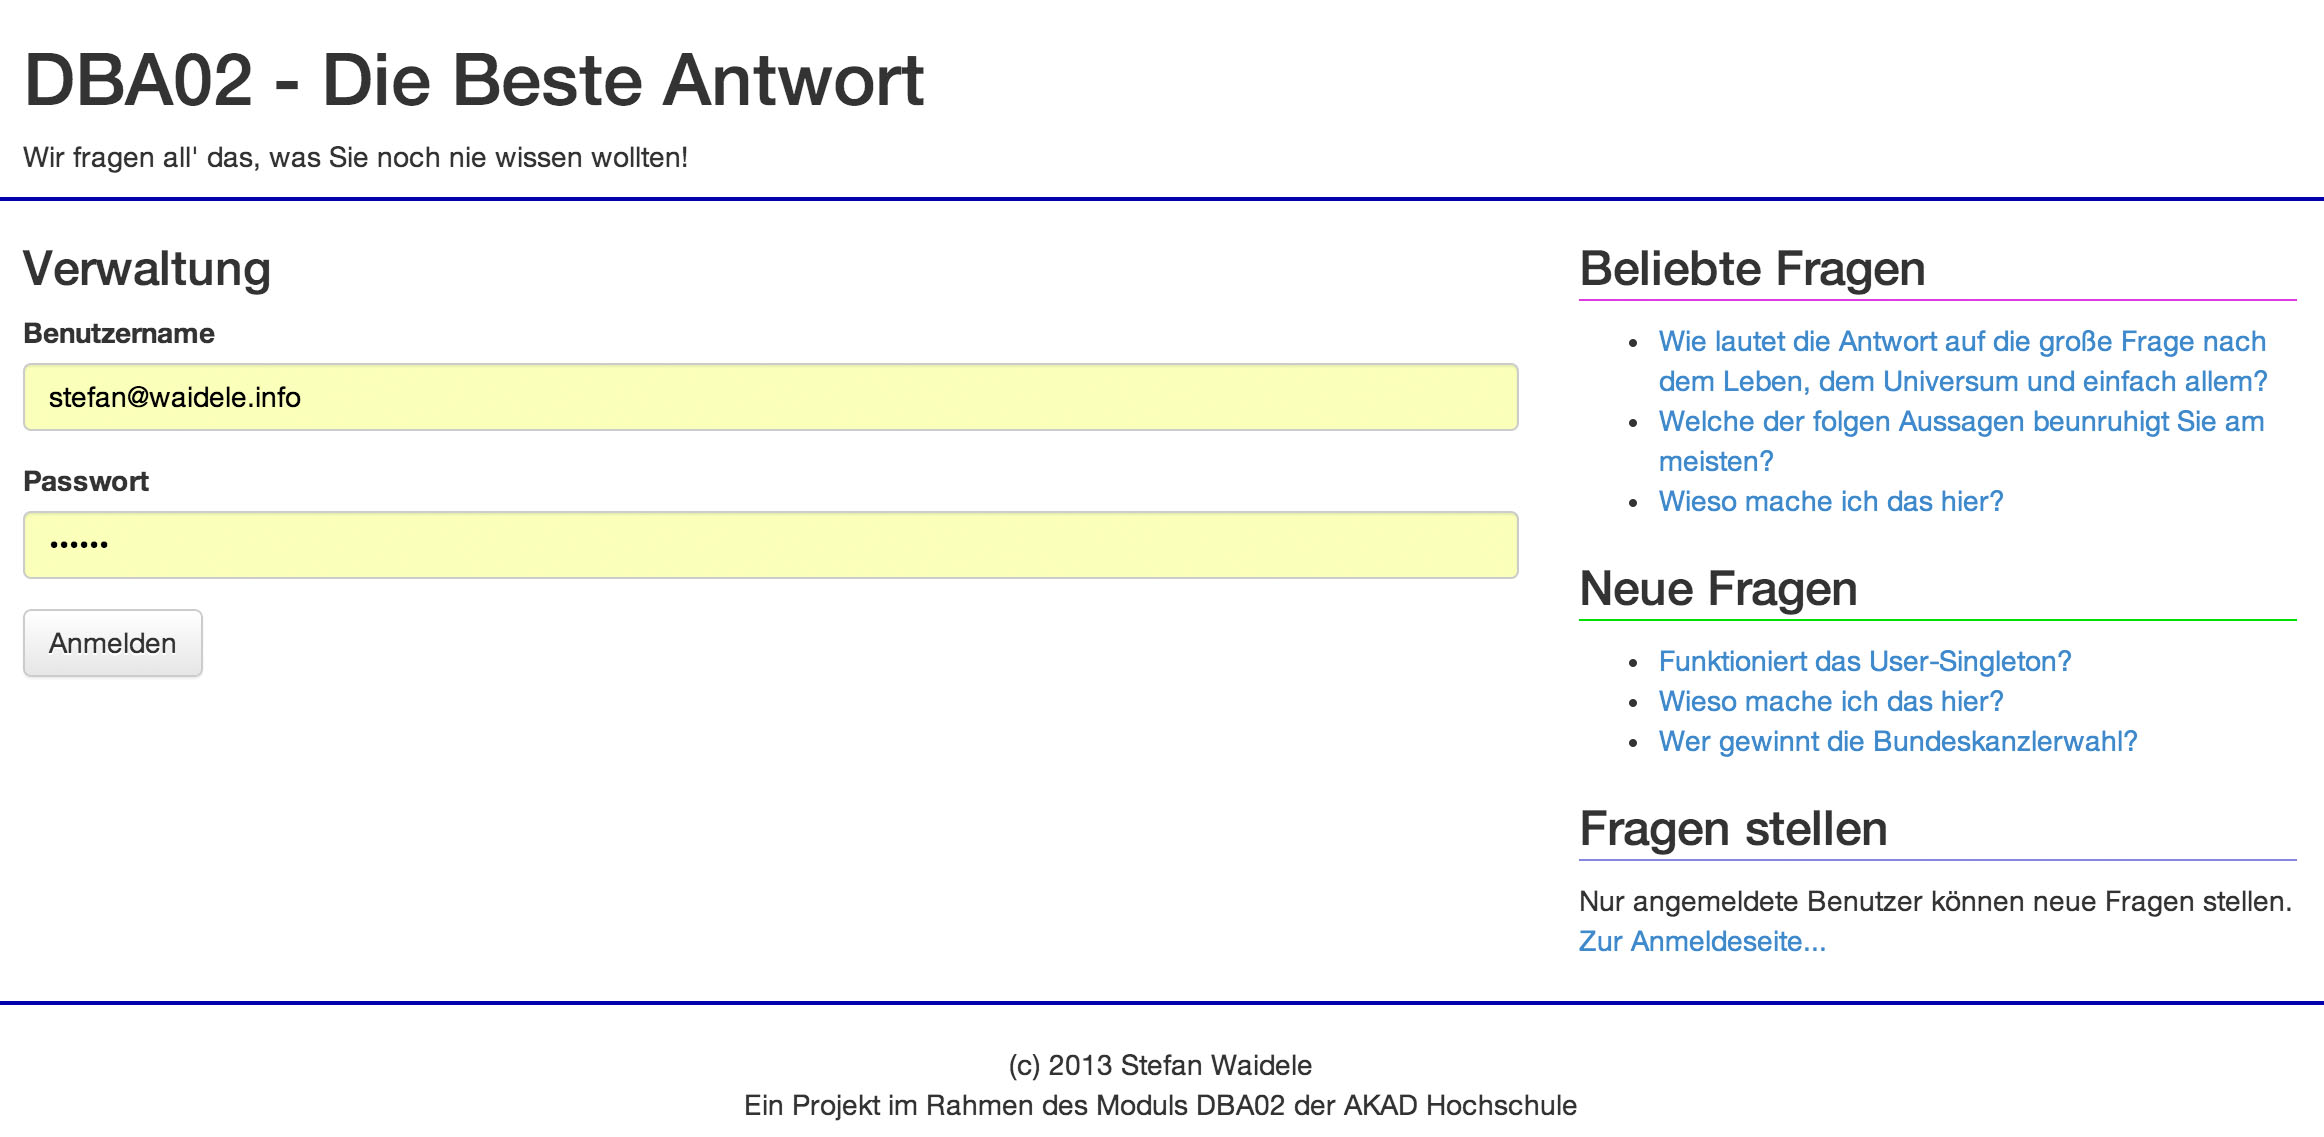
\includegraphics[width=\textwidth]{scr-anmeldung.jpg}
\caption{Screenshot: Anmeldung}
\label{scr:anmeldung}
\end{figure}

\begin{figure}[H]
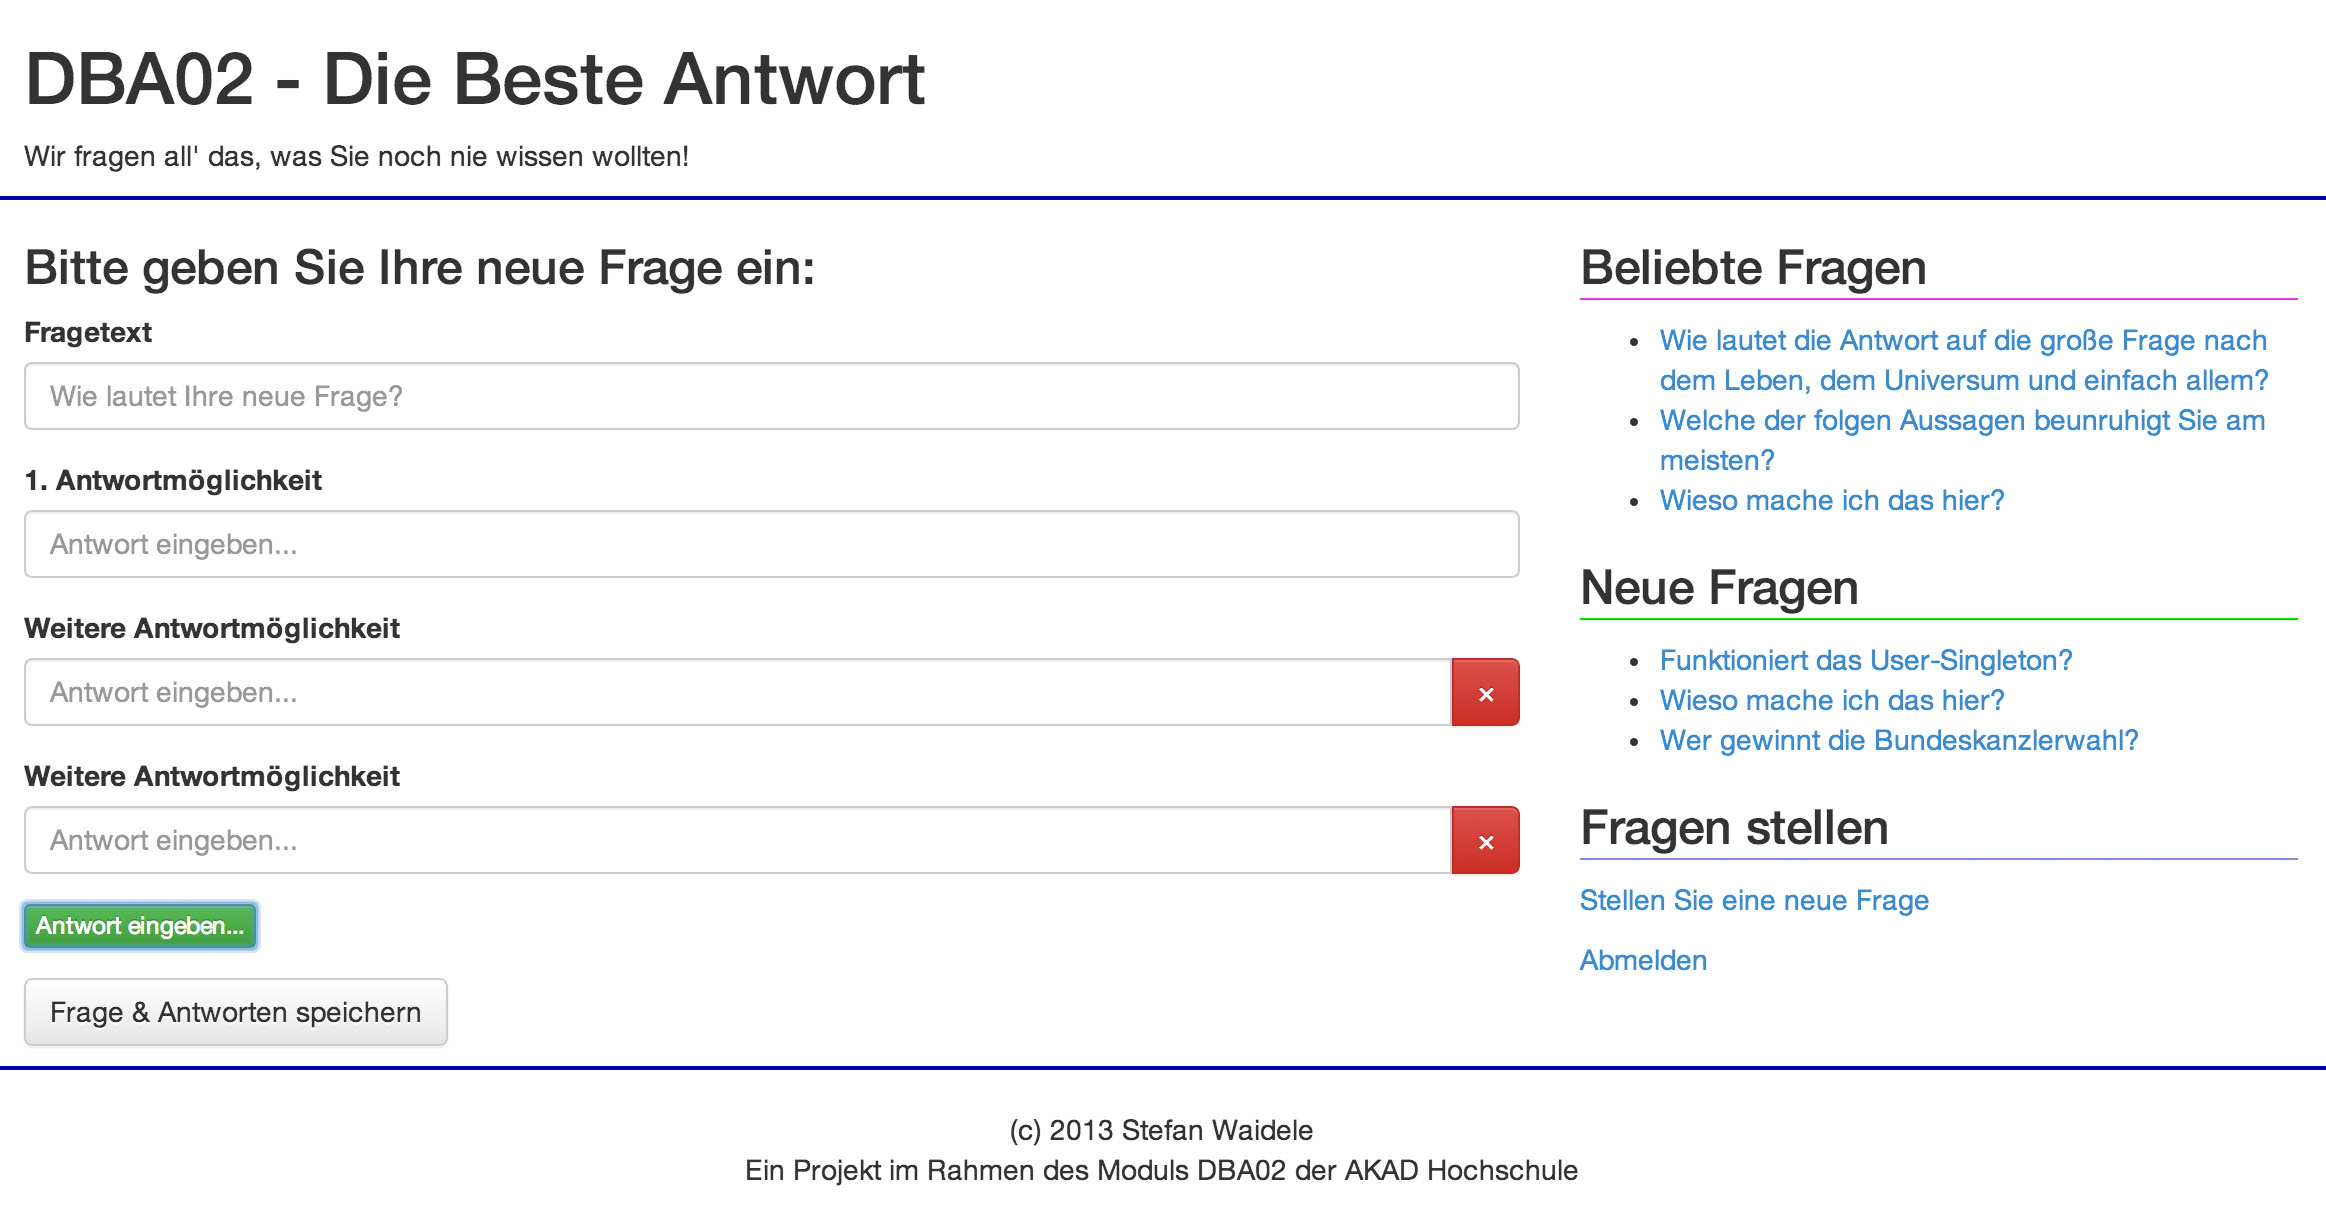
\includegraphics[width=\textwidth]{scr-neuefrage.jpg}
\caption{Screenshot: Neue Frage}
\label{scr:neuefrage}
\end{figure}

\section{Verzeichnisstruktur}

\begin{figure}[H]
\begin{spacing}{1.0}
\begin{minted}[bgcolor=bg]{bash}
\- bootstrap/:
|  |
|  \-- ...
|
\- class/:
|  |
|  \-- Datenbank.php
|  \-- SQL.php
|  \-- User.php
|
\- includes/:
|  |
|  \-- dbconf.ini
|  \-- footer.php
|  \-- header.php
|  \-- sidebar.php
|  
\- pages/:
|  |
|  \-- abmeldung.php
|  \-- anmeldung.php
|  \-- auswertung.php
|  \-- frage.php
|  \-- neuefrage.php
|  \-- speichern.php
| 
\- sql/:
|  |
|  \-- createdatabase.sql
|  \-- queries.sql
| 
\-- .htaccess
\-- index.php
\-- style.css
\end{minted}
\caption{Verzeichnisstruktur}
\label{bash:struktur}
\end{spacing}
\end{figure}

\section{Quellcode}

Der Quellcode der erstellten Anwendung befindet sich auf der diesem Assignment beigefügten CD--ROM. Außerdem steht er in der Modulspezifischen Arbeitsgruppe sowie unter \url{https://github.com/stwaidele/DBA02-Site} zur Verfügung.

\end{appendix}